\section{Analisi dei Risultati}
\subsection{VanillaCase}
\subsubsection{Risultati Co-Simulazione}
E' stata effettuata una simulazione nel caso base per accertarsi che il comportamento del sistema conduca alla convergenza delle due macchine.

\begin{figure}[h]
	\centering
	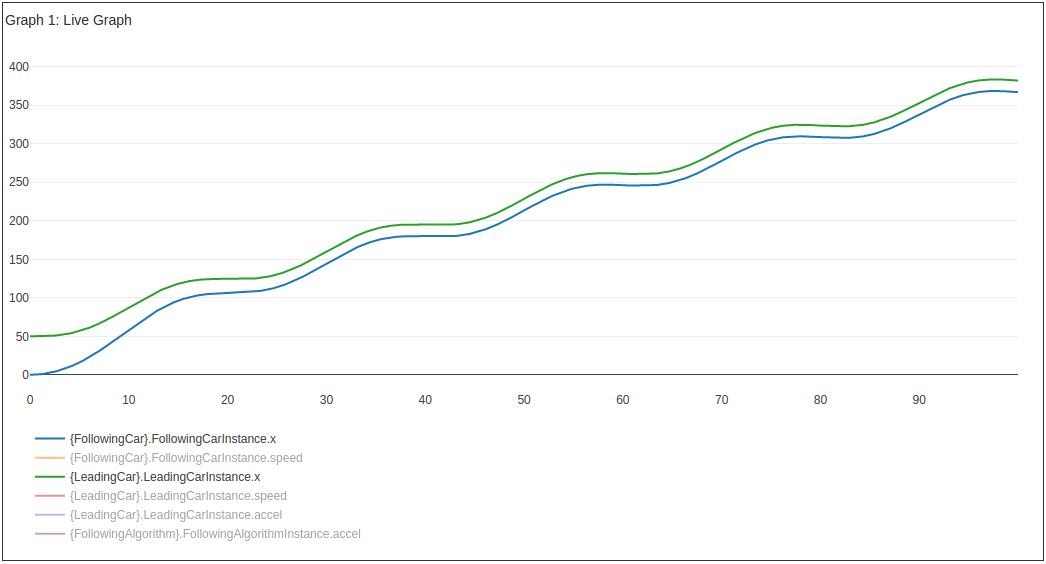
\includegraphics[width=\textwidth]{img/x.png}
	\caption{Posizione x della LeadingCar (verde) e FollowingCar (blu)}
\end{figure}

La distanze media tra le due auto è pari a \textbf{18.49m}. Dopo un iniziale periodo di transizione di circa 20s il sistema raggiunge la convergenza attesa e i due veicoli proseguono il percorso ad una distanza approssimativa di 15m fino a fine simulazione.

... immagine accel\_speed ...

Dalla figura sopra riportata è inoltre osservabile come negli istanti iniziali la following car abbia una accelerazione positiva maggiore di quella della leading. Questo si riflette inoltre sulle relative velocità. Il motivo di questo comportamento è dovuto all'iniziale periodo di transizione in cui la following car recupera la distanza iniziale (molto maggiore di 15m) dalla leading car. 

\subsection{Attacco all'accelerazione}
\subsubsection{Attacco Semplice}
\subparagraph{Risultati DSE}
Come primo approccio all'analisi al sistema è stato scelto di fare uso del DSE, configurato andando a variare l'\textbf{attack\_value} e l'\textbf{attack\_time} con i seguenti parametri::
\begin{itemize}
	\item \textbf{Attack\_value}: [-5, -1, 0, 1, 5]
	\item \textbf{Simulation\_time}: [0s, .., 40s] con step a 5
\end{itemize}
I risultati ottenuti sono stati successivamente eleborati così da estrapolare il seguente grafico che mostra la percentuale degli incidenti per ogni \textbf{attack\_value} al variare di \textbf{attack\_time}. Per individuare le condizioni di attacco è stato necessario estrapolare la distanza minima delle due macchine sull'intero tempo di simulazione.

\begin{figure}[H]
	\centering
	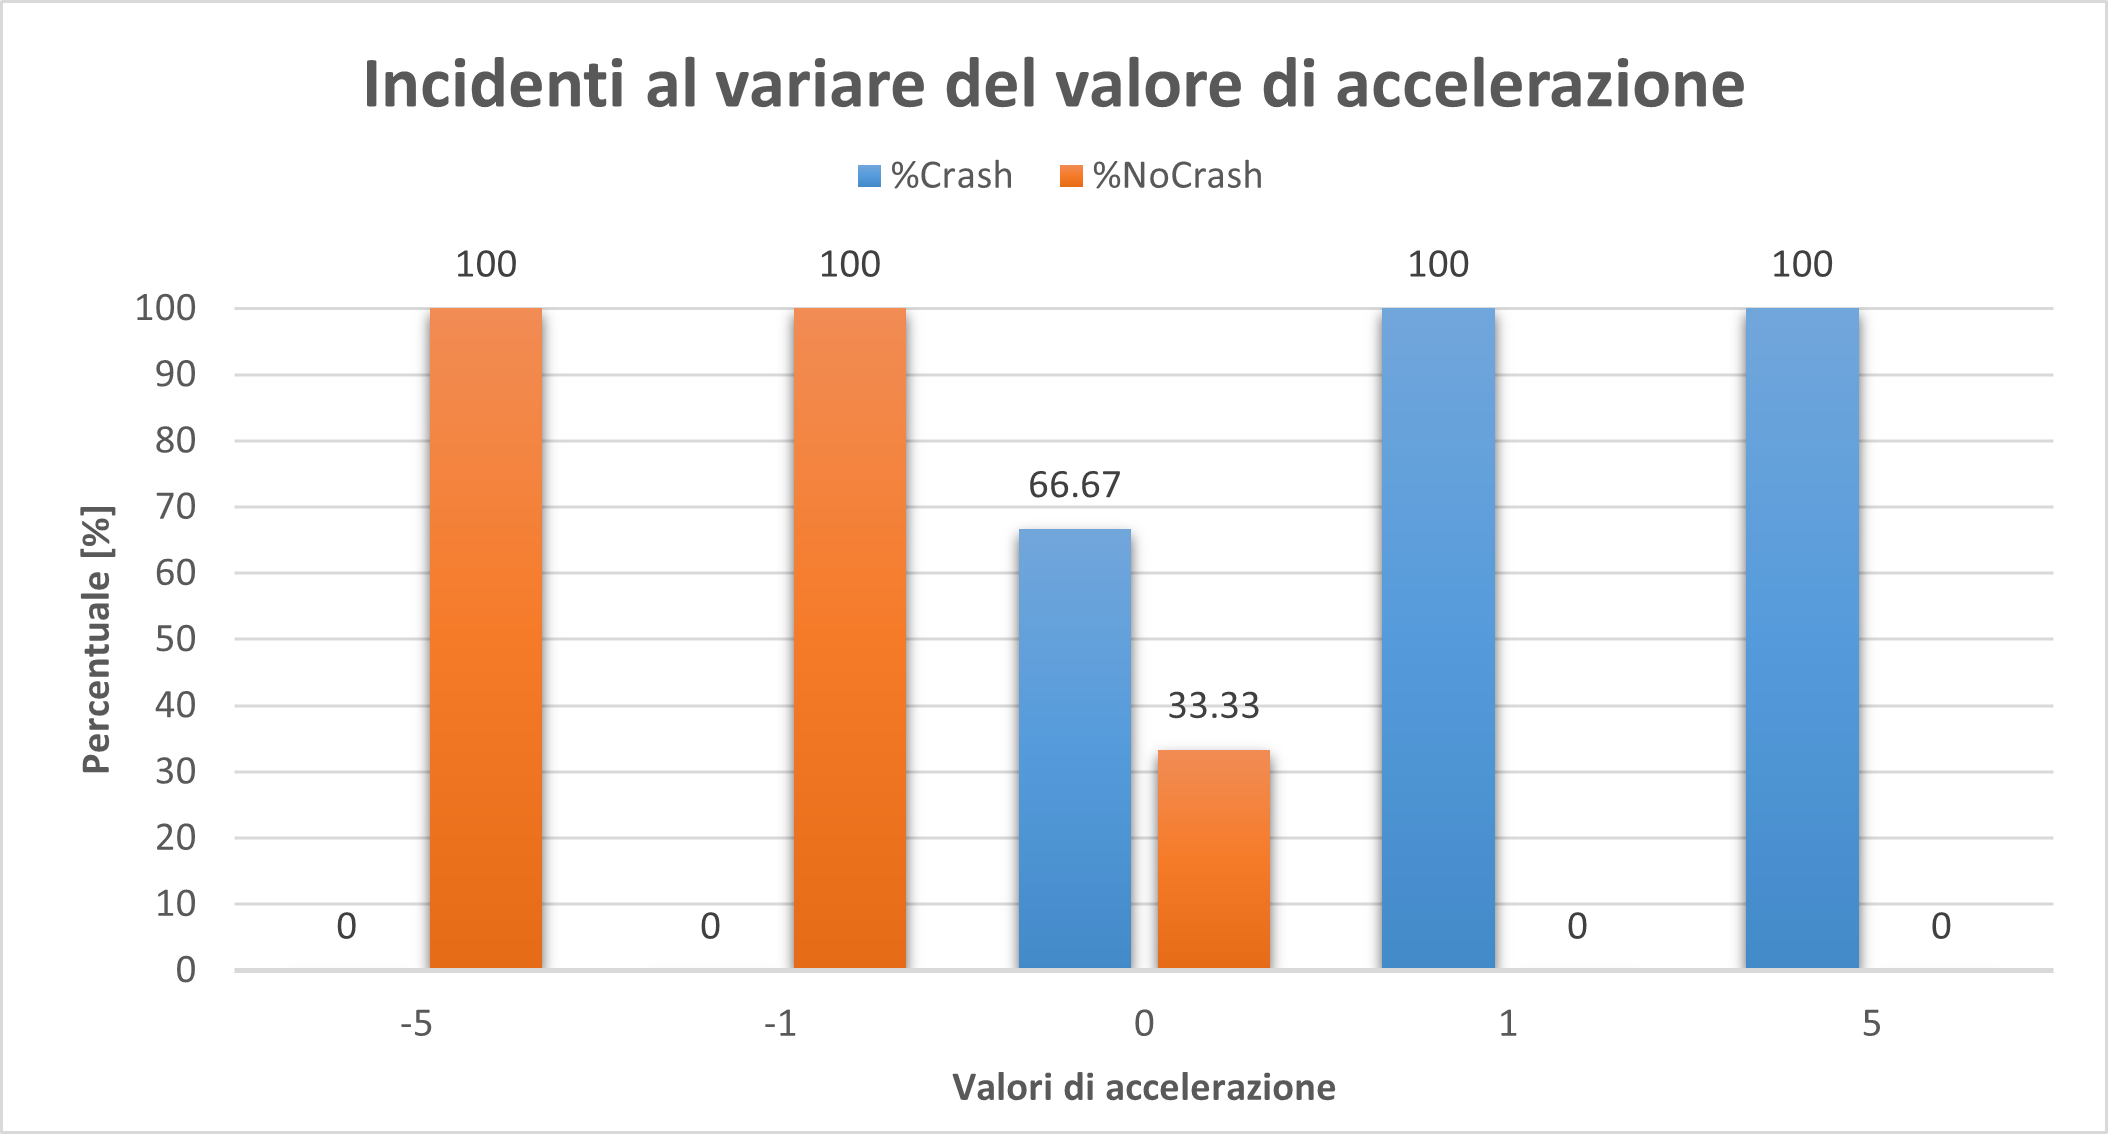
\includegraphics[width=\textwidth]{img/PlotPercentageIncidenteAttackAccel.png}
	\caption{Rappresentazione delle percentuali di incidenti nei casi testati con studio DSE}
\end{figure}


Come si può notare, è possibile individuare tre casi ben distinti:
\begin{itemize}
	\item \textbf{Attacchi con accelerazione negativa}: La following car è portata a rallentare con andamento lineare fino a cambiare la propria direzione di marcia. In questo caso le macchine tendono ad allontanarsi e l'incidente non avrà luogo. Inoltre è doveroso sottolineare che la following car perde completamente la capacità di inseguimento della leading car. Non ci sarà quindi convergenza fra following e leading car.
	\item \textbf{Attacchi con accelerazione pari a 0}: dal grafico emerge una chiara necessità di uno studio più approfondito di questa casistica in quanto non si delinea alcun risultato conclusivo. Essendo che l'accelerazione resta costante e pari a 0, la velocità della following car rimane costante al valore nel momento \textbf{Attack\_time}. La presenza o meno di incidenti dipende quindi proprio dal valore della velocità e quindi da \textbf{Attack\_time}
	\item \textbf{Attacchi con accelerazione positiva}: La following car è portata ad aumentare la propria velocità con andamento lineare . In questo caso le macchine tendono ad avvicinarsi e l'incidente avrà luogo.
\end{itemize}
Esistono tuttavia condizioni speciali che è doveroso sottolineare:
\begin{itemize}
	\item \textbf{Attacchi con accelerazione negativa}: Se la leading car decellerasse con continuità (per un intervallo di tempo sufficientemente ampio ) più di quanto non faccia la following car sotto attacco, allora in tal caso l'incidente avverrebbe
	\item \textbf{Attacchi con accelerazione positiva}: Se la leading car accelerasse con continuità (per un intervallo di tempo sufficientemente ampio ) più di quanto non faccia la following car sotto attacco, allora in tal caso l'incidente non avverrebbe
\end{itemize}
\subparagraph{Risultati Co-Simulazione}
Con l'obiettivo di rafforzare quanto appena descritto  e individuato tramite l'analisi dei risultati del DSE, vengono qui riportati tre casi fondamentali.
\subparagraph{Attacchi con accelerazione positiva pari a 1} Diseguito sono riportati i grafici in cui sono raffigurati l'attacco alle accelerazioni (Fig ...) e le posizioni dei due veicoli (Fig ...)
L'attacco è stato eseguito con:
\begin{itemize}
	\item \textbf{attack\_value}: 1
	\item \textbf{attack\_time}: 20s
\end{itemize}
........immagini......

Dalle osservazioni fatte si può evincere quanto segue:
**************************Da rivedere******************
\begin{itemize}
	\item La following car e la leading car fanno un incidente. Essendo che l'accelerazione è costante e tale che |Attack\_value| > 0 , allora la velocità tende ad aumentare linearmente. L'allontanamento da leading avverrà in modo quadratico nel tempo
	\item L'accellerazione che following algorithm pensa di dire a following car è sempre minore con andamento non lineare. Avrà sicuramente delle micro-oscillazioni ma sono quasi impercettibili a causa dell'elevata distanza dalla leading car. Quindi una decellerazione/accellerazione della leading car ha un effetto quasi trascurabile su following Algorithm
\end{itemize}

\subparagraph{Attacchi con accelerazione negativa pari a -1}
Diseguito sono riportati i grafici in cui sono raffigurati l'attacco alle accelerazioni (Fig ...) e le posizioni dei due veicoli (Fig ...)
L'attacco è stato eseguito con:
\begin{itemize}
	\item \textbf{attack\_value}: -1
	\item \textbf{attack\_time}: 20s
\end{itemize}
........immagini......

Dalle osservazioni fatte si può evincere quanto segue:
**************************Da rivedere******************
\begin{itemize}
	\item La following car non fa un incidente e continua la sua corsa in senso opposto rispetto alla leading car. Ogni considerazione fatta per il caso precedente rispetto a accelerazione e velocità sono ancora valide ma speculari.
	\item La velocità di following car decresce linearmente fino ad annullarsi e poi a cambiare segno (facendo muovere la macchina in retromarcia)
	\item Ogni considerazione fatta nel caso precedente rispetto all'accelerazione che following algorithm pensa di dire a following  car è tutt'ora valida e speculare al caso precedente.
\end{itemize}

\subparagraph{Attacchi con accelerazione pari a 0}


****************inserire una tabella****************

\subsubsection{Attacco Multiplo}
In questa sezione vengono riportati due diverse condizioni di attacco in cui quest'ultimo ha una durata di un certo numero di step e si ripete più volte nel tempo. L'obiettivo è quello di individuare una condizione in cui,nonostante gli attacchi ripetuti, il sistema risulta tollerante e uno invece in cui l'attacco porta a un incidente fra i due veicoli
\subparagraph{Risultati Co-Simulazione}
\subparagraph{Attacco senza incidente}
..............immagini + dati + spiegazione .............
\subparagraph{Attacco con incidente}
..............immagini + dati + spiegazione .............


\subsection{Attacco alla X}
\subparagraph{Attacco Semplice}
\subsubsection{Risultati Co-Simulazione}
Per cercare di dare un'interpretazione ai risultati del successivo studio verrà prima analizzato un caso d'esempio con i seguenti parametri:
\begin{itemize}
	\item \textbf{attack\_value}: 200
	\item \textbf{attack\_time}: 20s
\end{itemize}

Si ottiene il seguente plot:
\begin{figure}[H]
	\centering
	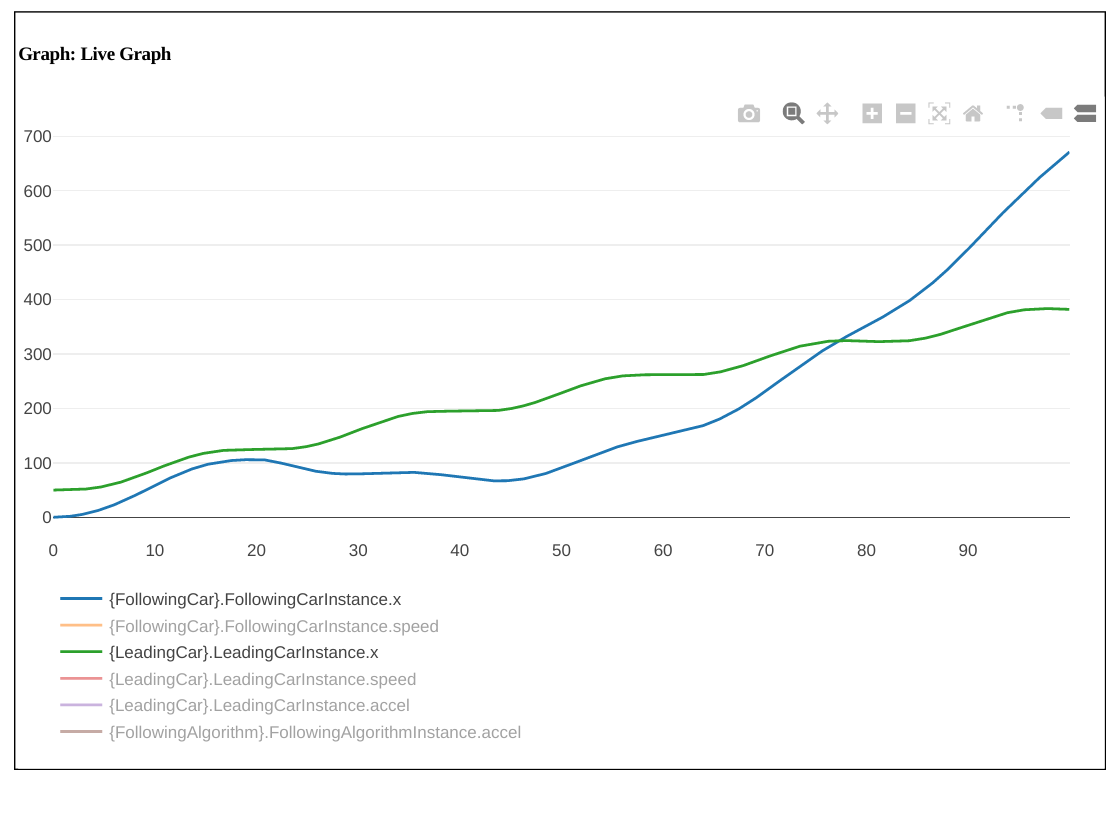
\includegraphics[width=\textwidth]{img/AttackXSimulation.png}
	\caption{Posizione x della LeadingCar (verde) e FollowingCar (blu)}
\end{figure}
Dal seguente risultato è possibile evincere tre differenti zone di comportamento della following car: nel \textbf{primo caso} nel quale l'attacco non viene ancora effettuato, la following car tende ad avvicinarsi alla leading car alla distanza configurata; nel \textbf{secondo caso}, dal un tempo di 20s ad uno di circa 40s, l'attacco inizierà ma la leading car non avrà superato ancora l'\textbf{attack\_value} impostato, che rappresenta la (alterata) posizione della following car: quest'ultima penserà di trovarsi davanti e decelererà; il \textbf{terzo caso}, dopo 40s, nel quale la leading car ha superato l'attack value e perciò la following car inizierà a riavvicinarsi fino all'impatto tra le due auto.
Per come è configurata la leading car, ovvero che tenderà sempre ad andare "in avanti" con qualche oscillazione nella velocità, è facile intuire che \textbf{un incidente con questo tipo di attacco per un tempo sufficiente avrà sempre luogo}, in quanto esisterà sempre un tempo nella quale la leading car supererà l'attack\_value, per quanto elevato possa essere quest'ultimo.  
\subsubsection{Risultati DSE}
E' stato studiato l'esito dell'attacco (INCIDENTE/NON INCIDENTE) andando a variare l'\textbf{attack\_value} e l'\textbf{attack\_time} con i seguenti parametri:
\begin{itemize}
	\item \textbf{Attack\_value}: [0 .. 200] con step a 1
	\item \textbf{Simulation\_time}: [50s, 100s]
\end{itemize}
 
 I risultati ottenuti possono essere riassunti nella seguente tabella
\begin{center}
	\begin{tabular}{ |p{6cm}|p{3cm}|p{4cm}|  }
		\hline
		Tempo di Simulazione& Attack Value & Risultato \\
		\hline
		\multirow{2}{4em}{50s} & [0, 149] & INCIDENTE \\
		& [150, 199] & NO INCIDENTE \\
		\hline
		\multirow{2}{4em}{100s} & [0, 199] & INCIDENTE \\
		& - & NO INCIDENTE \\
		\hline
	\end{tabular}
\end{center}
Come si può notare il tempo è una variabile importante per questo tipo di attacco, con un tempo sufficientemente alto l'attacco ha sempre luogo come detto in precedenza.

\subparagraph{Attacco Multiplo}
Sono stati individuati quattro diverse configurazioni che portano luogo a quattro classi di risultati diversi:
\begin{itemize}
	\item \textbf{Attack\_occurencies}: 3
	\item \textbf{Attack\_duration}: 2s
	\item \textbf{Attack\_time}: [30s, 50s, 70s]
	\item \textbf{Attack\_value}: 200
	\item \textbf{Attack\_distance}: 5s
	\item \textbf{Step\_size}: 0.01s
\end{itemize}
L'attacco pertanto avrà un pattern simile a livello temporale, la variabile è l'inizio dell'attacco stesso. I risultati degli esperimenti sono riassunti nella seguente tabella
\begin{center}
	\begin{tabular}{ |p{6cm}|p{3cm}| p{4cm}|  }
		\hline
		Attack Time & Distanza Minima & Risultato \\
		\hline
		30s & 14.9368 & NO INCIDENTE \\
		\hline
		50s & 0.639284 & NO INCIDENTE \\
		\hline
		70s & -20.38 & INCIDENTE \\
		\hline
	\end{tabular}
\end{center}
Una semplice interpretazione di questi risultati si basa sul fatto che il following algorithm produce un'accelerazione maggiore in caso la distanza tra le due auto sia maggiore: considerato che la distanza della following car vista dal following è fissa (per via dell'attacco in corso), nel caso il tempo di inizio sia maggiore, maggiore sarà la posizione della leading car e perciò maggiore sarà l'accelerazione in input che porterà ad una collisione nel caso di Attack time pari a 70s.